% Created 2018-12-12 Wed 08:52
% Intended LaTeX compiler: pdflatex
\documentclass[11pt]{article}
\usepackage[utf8]{inputenc}
\usepackage[T1]{fontenc}
\usepackage{graphicx}
\usepackage{grffile}
\usepackage{longtable}
\usepackage{wrapfig}
\usepackage{rotating}
\usepackage[normalem]{ulem}
\usepackage{amsmath}
\usepackage{textcomp}
\usepackage{amssymb}
\usepackage{capt-of}
\usepackage{hyperref}
\usepackage{minted}
\usepackage[1.0in]{geometry}
\author{Mijeong Ban}
\date{\today}
\title{}
\hypersetup{
 pdfauthor={Mijeong Ban},
 pdftitle={},
 pdfkeywords={},
 pdfsubject={},
 pdfcreator={Emacs 26.1 (Org mode 9.1.9)}, 
 pdflang={English}}
\begin{document}


\section*{Part One. Statistical Report}
\label{sec:org900f865}

\section*{Part Two. Textbook Exercises}
\label{sec:orgec46c72}
\subsection*{11.42 Relationships among PCB congeners}
\label{sec:org78a7acf}
Consider the following variables: PCB(the total amount of PCB) and four congeners: PCB52, PCB118, PCB138, and PCB180.
\subsubsection*{(a) Using numerical and graphical summaries, describe the distribution of each of these variables.}
\label{sec:org685646d}
\begin{table}[htbp]
\caption{Numerical Summaries}
\centering
\begin{tabular}{lrrrrrr}
Variable & Min & 1st Qu. & Median & Mean & 3rd Qu. & Max\\
\hline
PCB & 6.10 & 30.18 & 47.96 & 68.47 & 91.63 & 318.70\\
PCB52 & 0.020 & 0.228 & 0.477 & 0.958 & 0.892 & 9.060\\
PCB118 & 0.236 & 1.490 & 2.420 & 3.256 & 3.890 & 18.900\\
PCB138 & 0.640 & 3.180 & 4.920 & 6.827 & 8.650 & 32.300\\
PCB180 & 0.395 & 1.240 & 2.690 & 4.158 & 4.490 & 31.500\\
\end{tabular}
\end{table}

\begin{figure}[htbp]
\centering
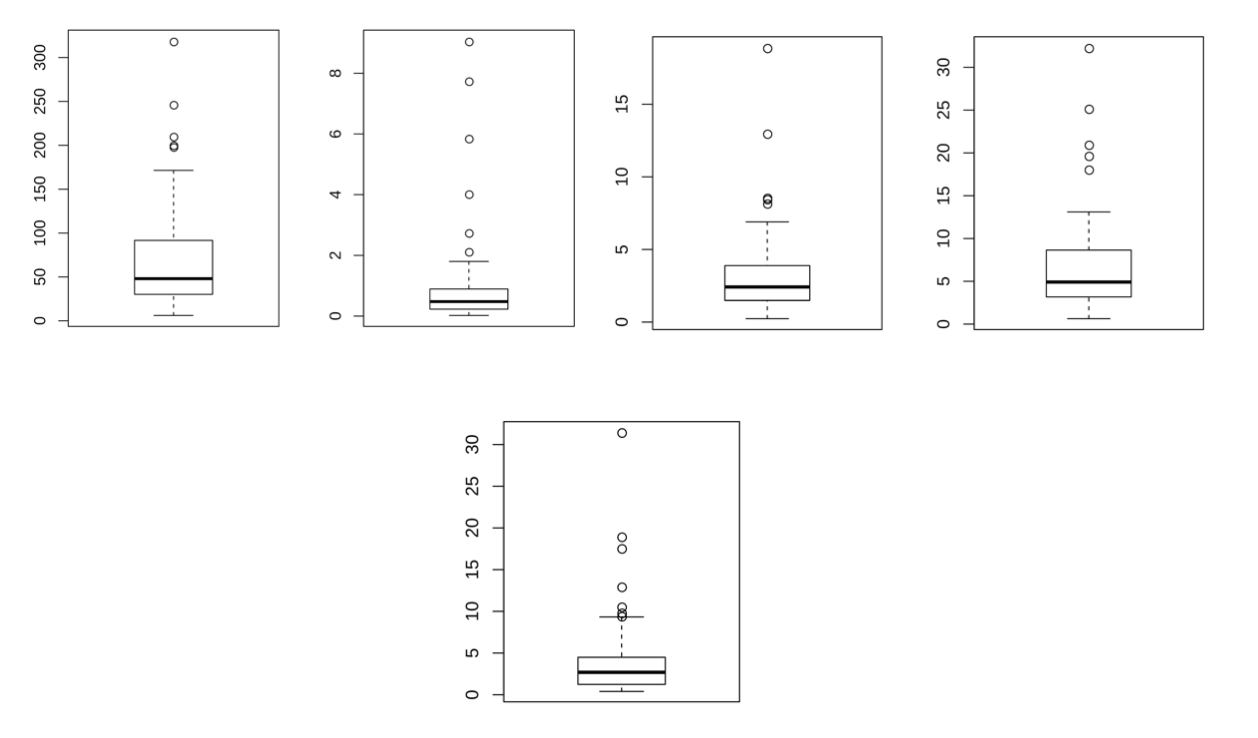
\includegraphics[width=.9\linewidth]{./graphs/image1.png}
\caption{Boxplots of PCB, PBC52, PCB118, PCB138 and PCB180}
\end{figure}
Figure 1 shows that the distribution of PCB and PCB180 is right skewed with about six outliers for both, while all the distribution of others are right skewed with about five outliers.  

\subsubsection*{(b) Using numerical and graphical summaries, describe the relationship between each pair of variables.}
\label{sec:orge0e174d}
\begin{table}[htbp]
\caption{Correlations}
\centering
\begin{tabular}{llr}
Variable 1 & Variable 2 & Correlation\\
\hline
PCB & PCB52 & 0.5963572\\
PCB & PCB118 & 0.843298\\
PCB & PCB138 & 0.9288353\\
PCB & PCB180 & 0.8008549\\
PCB52 & PCB118 & 0.6849073\\
PCB52 & PCB138 & 0.3008983\\
PCB52 & PCB180 & 0.08692971\\
PCB118 & PCB138 & 0.7293792\\
PCB118 & PCB180 & 0.4374443\\
PCB138 & PCB180 & 0.8823022\\
\end{tabular}
\end{table}
\end{document}
